\section{Simulación y modelado}
Antes de comenzar, se va a definir rápidamente los conceptos de simulación y modelado, ya que son la base de este proyecto. \\
El proceso de modelado se refiere a la extracción de conocimiento 
de un sistema físico que se desea simular, organizándolo de manera adecuada y representándolo de forma clara y sin ambigüedades. 
Por otro lado, el proceso de simulación hace referencia al desarrollo de experimentos sobre el modelo para hacer predicciones
sobre cómo se comportaría el sistema real si se fuesen a realizar los mismos experimentos sobre él  \cite{cellier2006}. \\


\section{Simulación de Sistemas Continuos}
Para el modelado del sistema físico, el siguiente proyecto adopta el paradigma de simulación de sistemas continuos. A diferencia de la simulación de eventos discretos, donde los cambios de estado ocurren de forma instantánea en momentos específicos, en un modelo continuo las variables del sistema evolucionan de manera ininterrumpida a lo largo del tiempo. Este comportamiento se define mediante sistemas de ecuaciones diferenciales ordinarias (ODE) y algebraicas diferenciales (DAE), las cuales describen las propiedades y la cinemática del modelo.\\


La elección de este enfoque es debido a la naturaleza dinámica de un vehículo. El comportamiento de un chasis involucra fenómenos físicos transitorios y de alta frecuencia, tales como la transferencia de carga, la compresión de los resortes de suspensión y el nivel de agarre variable. Es fundamental que el estado físico del vehículo esté definido para cualquier instante arbitrario $t$. Si no se garantizara esta continuidad matemática, se producirían vacíos de información o discontinuidades artificiales que alterarían las fuerzas resultantes, provocando inestabilidad numérica y un comportamiento dinámico completamente irreal. \\

\subsection{Modelos de ecuaciones diferenciales ordinarias (ODE)}

La forma más elemental de describir un sistema continuo es el modelo explícito de ecuaciones diferenciales ordinarias, también conocido como ODE o modelo en espacio de estados \cite{cellier2006}:
\begin{equation}
	\dot{\mathbf{x}}(t) = \mathbf{f}\bigl(\mathbf{x}(t), \mathbf{u}(t), t\bigr), \qquad \mathbf{x}(t_0) = \mathbf{x}_0
	\label{eq:state_space}
\end{equation}

$\mathbf{x}$ es el vector de estado,  $\mathbf{u}$ el vector de entradas y $t$ representa el tiempo. Las variables que se quieren observar como resultado de la simulación se obtienen mediante ecuaciones de salida que dependen únicamente de los estados y las entradas, $\mathbf{y} = \mathbf{g}(\mathbf{x}, \mathbf{u}, t)$. \\

Las variables de estado son las salidas de los integradores del modelo. No es el modelo quien las calcula, sino el algoritmo de integración numérica, el modelo solo debe proveer las derivadas de los estados  $\dot{\mathbf{x}}$. El modelo calcula $\dot{\mathbf{x}}(t_k)$ a partir de $\mathbf{x}(t_k)$, y el algoritmo de integración calcula $\mathbf{x}(t_{k+1})$ a partir de ambos \cite{cellier2006}.

Mientras $\mathbf{f}$ y sus derivadas no presenten discontinuidades, cada trayectoria de estado $x_i(t)$ es una función continua del tiempo, y puede aproximarse mediante un desarrollo en serie de Taylor alrededor de cualquier punto de la trayectoria:
\begin{equation}
	x_i(t^* + h) = x_i(t^*) + f_i(t^*)\cdot h + \frac{d f_i(t^*)}{dt}\cdot\frac{h^2}{2!} + \dots
\end{equation}
Los distintos algoritmos de integración difieren en cómo aproximan las derivadas de orden superior y en la cantidad de términos de la serie que consideran \cite{cellier2006}.

\subsection{Modelos de ecuaciones algebraico-diferenciales (DAE)}
\label{sec:dae_section}
Para muchos sistemas físicos no resulta sencillo ni natural formular el modelo como un sistema ODE. Lo habitual es obtener un conjunto de ecuaciones en el que las derivadas de los estados aparecen de forma implícita, mezcladas con ecuaciones algebraicas. A este tipo de descripciones se las denomina ecuaciones algebraico-diferenciales (DAE) y en su forma implícita más general se escriben como \cite{cellier2006}:

\begin{equation}
	\mathbf{f}\bigl(\mathbf{x}, \dot{\mathbf{x}}, \mathbf{u}, t\bigr) = \mathbf{0}
	\label{eq:implicit_dae}
\end{equation}

El modelado orientado a objetos de sistemas físicos conduce a descripciones DAE implícitas. Cada componente aporta sus propias ecuaciones constitutivas y las conexiones entre componentes agregan más ecuaciones de acoplamiento. El resultado es un sistema en el cual ninguna ecuación indica qué variable debe calcularse a partir de ella \cite{cellier2006}. En este estado las ecuaciones son acausales, es decir, el signo igual expresa una igualdad y no una asignación. \\

%El modelado orientado a objetos de sistemas físicos conduce invariablemente a descripciones DAE implícitas. Cada componente aporta sus propias ecuaciones constitutivas, y las conexiones entre componentes aportan ecuaciones adicionales de acoplamiento; el resultado es un sistema extenso en el que ninguna ecuación indica qué variable debe calcularse a partir de ella \cite{cellier2006}. En este estado las ecuaciones son \textit{acausales}: el signo igual expresa una igualdad y no una asignación. Esto refleja una propiedad de la física misma, en la que la causalidad computacional de una ley no está predeterminada. En una resistencia, por ejemplo, no puede afirmarse que la corriente provoque la caída de tensión ni que la diferencia de potencial provoque la corriente; ambas son aspectos simultáneos de un mismo fenómeno, y según el contexto el cálculo deberá adoptar una u otra dirección \cite{cellier2006}. \\


Un modelo DAE implícito puede convertirse en uno explícito decidiendo qué variable se despeja de cada ecuación (ordenamiento horizontal) y ordenando las ecuaciones de modo que ninguna variable se utilice antes de ser calculada (ordenamiento vertical). Después de aplicar este proceso, cada incógnita aparece exactamente una vez, a la izquierda del signo igual y estos pasan a funcionar como asignaciones. Si después se sustituyen las ecuaciones explícitas hasta que las derivadas de los estados dependan únicamente de los estados y las entradas, se obtiene el modelo ODE de la Ecuación (2.1) \cite{cellier2006}. Existen algoritmos que realizan este ordenamiento de forma automática, como las variantes del algoritmo de Tarjan \cite{cellier2006}. \\

Sin embargo, no todo sistema DAE puede ordenarse por completo. Pueden aparecer dos tipos de dificultades estructurales \cite{cellier2006}:

\begin{itemize}

	
	\item \textbf{Lazos algebraicos:} Subconjuntos de ecuaciones en los que cada ecuación y cada incógnita resultante dependen de al menos otras dos, por lo que no es posible despejarlas individualmente y deben resolverse al mismo tiempo, ya sea simbólicamente o mediante iteración numérica.
	
	\item \textbf{Singularidades estructurales:} Situaciones en las que existen restricciones algebraicas entre variables de estado, por lo que no son independientes entre sí y el sistema tiene menos grados de libertad que los integradores.
\end{itemize}

Estas dificultades se miden usando el índice de perturbación del sistema. Un DAE de índice $0$ no contiene lazos algebraicos ni singularidades estructurales, uno de índice $1$ tiene lazos algebraicos pero no singularidades y uno de índice mayor a $1$ (también conocido como DAE de índice superior) contiene singularidades estructurales  \cite{cellier2006}. Existen algoritmos de reducción de índice, como el de Pantelides que diferencian simbólicamente las ecuaciones de restricción para disminuir el índice del sistema en una unidad por aplicación del algoritmo. \\

Una vez formulado un modelo DAE, existen dos caminos para simularlo: convertirlo en un modelo ODE explícito que luego se integra con los métodos numéricos tradicionales o resolverlo directamente con un solver de DAE. En este último caso, al aplicar una fórmula de integración implícita a la ecuación (2.3), las derivadas $\dot{\mathbf{x}}_{k+1}$ se expresan en función de los estados, y el paso de integración se reduce a un sistema de ecuaciones no lineales $\mathbf{F}(\mathbf{x}_{k+1}) = \mathbf{0}$ \cite{cellier2006}. \\

%Una vez formulado un modelo DAE, existen dos caminos para simularlo: convertirlo simbólicamente en un modelo ODE explícito que luego se integra con los métodos numéricos tradicionales, o resolverlo directamente con un \textit{solver} de DAE. En este último caso, al aplicar una fórmula de integración implícita a la Ecuación~\eqref{eq:implicit_dae}, las derivadas $\dot{\mathbf{x}}_{k+1}$ se expresan en función de los estados, y el paso de integración se reduce a un sistema de ecuaciones no lineales $\mathbf{F}(\mathbf{x}_{k+1}) = \mathbf{0}$ que se resuelve por iteración de Newton \cite{cellier2006}. \\

Esto resulta relevante para los sistemas mecánicos multicuerpo. Formular un modelo ODE de un sistema de este estilo no es práctico, mientras que un modelo DAE es relativamente sencillo de obtener, alcanza con describir la dinámica de cada cuerpo por separado y agregar las interacciones entre ellos como ecuaciones de restricción. Este procedimiento suele dar lugar a modelos de índice $3$ con restricciones no lineales, en especial si hay topologías con bucles cinemáticos cerrados \cite{cellier2006}. Además, la cantidad de ecuaciones depende fuertemente de la elección de variables de estado, una elección descuidada puede hacer que crezca con la cuarta potencia de la cantidad de articulaciones, mientras que una elección adecuada logra que crezca solo linealmente \cite{cellier2006}.\\

%Esta distinción resulta particularmente relevante para los sistemas mecánicos multicuerpo. Formular un modelo ODE de un sistema multicuerpo complejo no es práctico, mientras que un modelo DAE es relativamente sencillo de obtener: basta con describir la dinámica de cada cuerpo por separado y agregar las interacciones entre ellos como ecuaciones de restricción. No obstante, este procedimiento suele dar lugar a modelos de índice~3 con restricciones fuertemente no lineales, en especial en topologías con lazos cinemáticos cerrados \cite{cellier2006}. Además, la cantidad de ecuaciones resultante depende fuertemente de la elección de las variables de estado: una elección descuidada puede hacer que crezca con la cuarta potencia de la cantidad de articulaciones, mientras que una elección adecuada logra que crezca solo linealmente. Por este motivo, la biblioteca multicuerpo desarrollada por Martin Otter no recurre al algoritmo de Pantelides, sino que formula sus ecuaciones de modo que las singularidades estructurales queden resueltas desde la propia formulación del modelo \cite{cellier2006}. \\

\subsection{Solvers}

Como se mencionó anteriormente, una vez traducido y compilado, el conjunto de componentes del sistema de simulación pasa a un sistema de ecuaciones algebraico-diferenciales (DAE). La integración de este sistema en el tiempo no puede realizarse de forma analítica, por lo que se recurre a métodos de integración numérica (\textit{solvers}). En el marco de OpenModelica se evaluaron dos solvers de referencia para la ejecución de la simulación: DASSL y CVODE. Ambos comparten la característica de ser especialmente adecuados para sistemas \textit{rígidos} (\textit{stiff}), condición que presenta el modelo del vehículo debido a la coexistencia de dinámicas de muy distinta escala temporal. A continuación se va a explicar el funcionamiento de ambos, lo cual va a resultar necesario para comprender esta tesina.

\subsubsection*{DASSL}

DASSL (\textit{Differential/Algebraic System Solver}) es el solver por defecto de OpenModelica, desarrollado por Petzold en Sandia National Laboratories \cite{petzold1982}. La principal ventaja es que opera directamente sobre la forma implícita  $F(t, y, \dot{y}) = 0$, más general que la forma explícita estándar $\dot{y} = f(t, y)$, lo que lo hace más apto ante sistema DAE como los que surgen del análisis dinámico de sistemas mecánicos multicuerpo. En particular, DASSL es aplicable incluso  cuando la matriz jacobiana $\partial F / \partial \dot{y}$ es singular, situación habitual en presencia de restricciones algebraicas.


El algoritmo se basa en la idea de Gear de reemplazar la derivada $\dot{y}$ en la ecuación implícita por una aproximación en diferencias, y resolver la ecuación no lineal resultante en el instante actual $t_n$ mediante el método de Newton. Para ello, emplea la fórmula de diferenciación regresiva (\textit{Backward Differentiation Formula}, BDF) de orden $k$, con $k$ variable entre $1$ y $5$. En su forma más simple, de primer orden, la aproximación es:

\begin{equation}
	F\!\left(t_n,\, y_n,\, \frac{y_n - y_{n-1}}{\Delta t_n}\right) = 0
\end{equation}

En cada paso, DASSL selecciona automáticamente tanto el orden $k$ como el tamaño de paso $\Delta t_n$ en función del comportamiento de la solución y de una estimación del error local de truncamiento, empleando además una formulación BDF de coeficiente líder fijo (\textit{fixed-leading-coefficient}) que mejora la estabilidad numérica. La ecuación no lineal se resuelve con una variante del método de Newton cuya matriz de iteración,

\begin{equation}
	G = \frac{\partial F}{\partial \dot{y}} + \alpha\, \frac{\partial F}{\partial y}
\end{equation}

donde $\alpha$ es un escalar que depende del paso y el orden. se factoriza y se reutiliza durante tantos pasos como sea posible para reducir el coste computacional. Su robustez frente a la forma DAE completa lo convierte en la opción de referencia para la validación del modelo.

\subsubsection*{CVODE}

CVODE (\textit{C-language Variable-coefficient ODE solver}) fue desarrollado por Cohen y Hindmarsh en Lawrence Livermore National Laboratory como una reescritura en C de los paquetes VODE y VODPK, y forma parte de la suite SUNDIALS \cite{cohen1995}. A diferencia de DASSL, CVODE resuelve el problema de valor inicial de forma explícita $\dot{y} = f(t, y)$, por lo tanto, para su uso, el compilador de OpenModelica debe reducir previamente el sistema DAE a una forma de estado equivalente (índice 1 o forma ODE), operación que se apoya en la reducción de índice que aportan los ensamblajes analíticos de las suspensiones.

CVODE resuelve tanto sistemas rígidos como no rígidos mediante dos familias de métodos lineales multipaso de coeficiente, orden y paso variable: las fórmulas de Adams-Moulton (para problemas no rígidos, con orden entre $1$ y $12$) y las fórmulas BDF (para problemas rígidos, con orden entre $1$ y $5$). Ambas familias se expresan en la forma general:

\begin{equation}
	\sum_{i=0}^{K_1} \alpha_{n,i}\, y_{n-i} + h_n \sum_{i=0}^{K_2} \beta_{n,i}\, \dot{y}_{n-i} = 0
\end{equation}

donde para el caso BDF se tiene $K_1 = q$ y $K_2 = 0$, siendo $q$ el orden. En cada paso debe resolverse un sistema no lineal, que CVODE aborda mediante iteración funcional (para el caso no rígido, sin resolución de sistemas lineales) o mediante iteración de Newton (para el caso rígido). En este último caso, la iteración de Newton requiere resolver sistemas lineales con la matriz:

\begin{equation}
	M \approx I - \gamma\, J, \qquad J = \frac{\partial f}{\partial y}, \qquad \gamma = h_n\, \beta_{n,0}
\end{equation}

Para el tratamiento del jacobiano $J$ en el caso rígido, CVODE ofrece varias opciones: tratamiento denso, en banda, diagonal aproximado, o un método iterativo de Krylov (GMRES precondicionado), lo que le confiere gran flexibilidad y eficiencia. Su arquitectura modular, en la que el integrador principal es independiente del solver lineal empleado, junto con su condición de código moderno y activamente mantenido, lo convierten en una alternativa atractiva a DASSL para la búsqueda de un rendimiento adecuado en la ejecución en tiempo real.\\


\subsection{Manejo del reloj}

En una simulación, el tiempo no pasa por sí solo, el usuario tiene que especificar cuándo y cómo sucede. Dependiendo de cómo se controla este reloj pueden haber efectos en la eficiencia y fidelidad de la simulación \cite{cellier2006}.\\

Una computadora digital no tiene forma de calcular cualquier valor de una función real en un valor de tiempo real. Lo que se hace para evitar esto es discretizar el eje que representa el tiempo en la simulación, de forma que la cantidad de puntos discretos es finita y la simulación procede saltando entre estos puntos que representan al tiempo \cite{cellier2006}. A mayor cantidad de puntos generados, la fidelidad de la simulación aumenta, a cambio de tiempo de procesamiento que se gasta calculando esos valores extra.\\

Dentro de la simulación, el modelo se vuelve a convertir reduciendo las ecuaciones diferenciales a ecuaciones en diferencias ($\Delta E$), convirtiendo modelos ODE explícitos a modelos  $\Delta E$ y modelos DAE implícitos a modelos $\Delta AE$ \cite{cellier2006}.\\

% Inside the simulation box, the model gets converted once more by reducing differential equation models to difference equation (ΔE) models. Thereby, an explicit ODE model is converted to an explicit ΔE model, whereas an implicit DAE model is converted to an implicit ΔAE model, etc.

%A digital computer has no means of computing numerically any real-valued function of a real–valued argument. To do so would require an infinite amount of real time. Instead, the time axis in the simulation must be discretized, such that the total number of discrete time points within the range of simulated time remains finite, and the simulation must proceed by jumping from one discrete time point to the next. 


%Cabe destacar que, si bien el modelo teórico es de naturaleza continua, su resolución en un entorno de hardware digital requiere la aplicación de métodos de integración numérica (solvers). Estos métodos calculan el estado continuo del sistema aproximándolo en intervalos o pasos de tiempo computacionales (time steps) lo suficientemente pequeños como para garantizar tanto la fidelidad física como la ejecución del sistema en tiempo real.

%%%%%%%%%%%%%%


%Cabe destacar que, si bien el modelo teórico es de naturaleza continua, su resolución en un entorno de hardware digital requiere la aplicación de métodos de integración numérica (solvers). Estos métodos calculan el estado continuo del sistema aproximándolo en intervalos o pasos de tiempo computacionales (time steps) lo suficientemente pequeños como para garantizar tanto la fidelidad física como la ejecución del sistema en tiempo real.

%La elección de este enfoque es debido a la naturaleza dinámica de un vehículo. El comportamiento de un chasis involucra fenómenos físicos transitorios y de alta frecuencia, tales como la transferencia de carga, la compresión de los resortes de suspensión y el nivel de agarre variable. Es fundamental que el estado físico del vehículo esté definido para cualquier instante arbitrario $t$. Si no se garantizara esta continuidad matemática, se producirían vacíos de información o discontinuidades artificiales que alterarían las fuerzas resultantes, provocando inestabilidad numérica y un comportamiento dinámico completamente irreal. \\

%Cabe destacar que, si bien el modelo teórico es de naturaleza continua, su resolución en un entorno de hardware digital requiere la aplicación de métodos de integración numérica (solvers). Estos métodos calculan el estado continuo del sistema aproximándolo en intervalos o pasos de tiempo computacionales (time steps) lo suficientemente pequeños como para garantizar tanto la fidelidad física como la ejecución del sistema en tiempo real.

\section{Lenguaje Modelica}
Para la implementación del modelo continuo se adoptará Modelica, un lenguaje de modelado orientado a objetos diseñado para la representación de sistemas físicos dinámicos complejos. Este lenguaje proporciona herramientas nativas que permiten definir tanto las ecuaciones intrínsecas de cada componente como las relaciones estructurales (topología) que rigen la interacción y el acoplamiento entre dichos componentes.\\

Si bien Modelica comparte similitudes sintácticas y de encapsulamiento con lenguajes de programación orientados a objetos tradicionales, como C++ o Python, difiere de estos en dos aspectos computacionales fundamentales. En primer lugar, es estrictamente un lenguaje de modelado: sus clases no generan secuencias de instrucciones ejecutables de manera directa, sino que se traducen en sistemas de ecuaciones que posteriormente son resueltos por un motor de simulación. En segundo lugar, Modelica emplea un paradigma declarativo, en lugar de asignar valores a variables mediante algoritmos paso a paso, el desarrollador plantea igualdades matemáticas donde la dirección del flujo de datos no está predefinida, siendo el compilador el encargado de analizar y determinar la causalidad algorítmica necesaria para su resolución.\\

\subsection{Desarrollo de un modelo en Modelica}
En esta sección se va a explicar cómo se desarrolla un modelo en Modelica. Para este ejemplo, se van a utilizar elementos de la Modelica Standard Library, una librería abierta y gratuita desarrollada por la Modelica Association, que incluye, entre otras cosas, elementos para construir sistemas mecánicos, eléctricos, magnéticos, térmicos, de fluidos y de control \cite{msl}.

\begin{figure}[htbp]
	\centering
	% Replace 'example-image' with your file name
	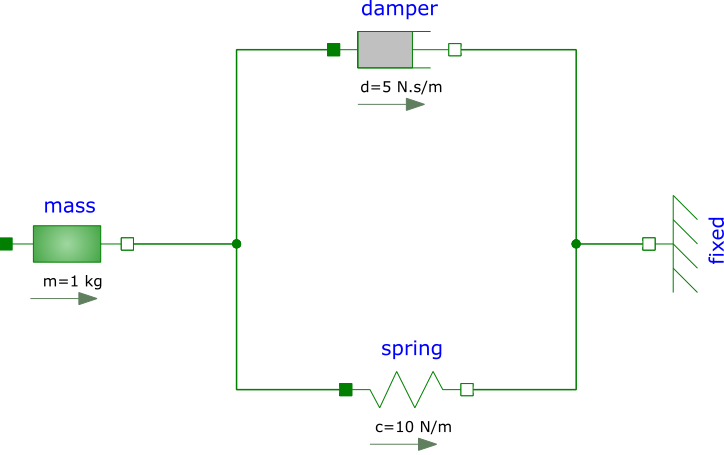
\includegraphics[width=1\textwidth]{img/Example.png} 
	
	\vspace{1em} % Adds spacing between image and quote
	
	\caption[Modelo de ejemplo en Modelica]{Gráfico de bloques de un sistema resorte-amortiguador creado y exportado como SVG desde OpenModelica.}
	\label{fig:example}
\end{figure}




\newpage

\begin{lstlisting}[caption={Código del ejemplo resorte-amortiguador}, label={lst:example}]
model Example
	Modelica.Mechanics.Translational.Components.Mass mass(m = 1);
	Modelica.Mechanics.Translational.Components.Fixed fixed;
	Modelica.Mechanics.Translational.Components.Damper damper(d = 5);
	Modelica.Mechanics.Translational.Components.Spring spring(s_rel(start = 0), c = 10, s_rel0 = 2);
equation
	connect(mass.flange_b, damper.flange_a);
	connect(damper.flange_b, fixed.flange;
	connect(spring.flange_a, mass.flange_b);
	connect(spring.flange_b, fixed.flange);
end Example;
\end{lstlisting}

En la figura~\ref{fig:example} se muestra un modelo de ejemplo desarrollado en OpenModelica, representa a una masa de $1$ kg conectada a un sistema resorte-amortiguador de una dimensión. El modelo está compuesto de otros modelos que se usan como base, particularmente, se están utilizando los modelos \textit{Mass}, \textit{Damper}, \textit{Spring} y \textit{Fixed}. Cada uno de estos modelos tiene sus ecuaciones constitutivas, y se conectan entre ellos mediante conectores denominados \textit{flange} (en el caso de un sistema de una dimensión translacional). \\

El gráfico representa la \textit{Diagram View} o vista de diagrama, que es una herramienta visual para crear modelos en la cual los objetos simplemente se arrastran al diagrama y se conectan de forma interactiva, sin embargo, esto es solamente una interfaz gráfica que funciona como frente ante el código en Modelica. El código~\ref{lst:example} es la traducción de la figura~\ref{fig:example} a lenguaje Modelica, esto se hace automáticamente y ambas representaciones son equivalentes y válidas por sí mismas. Este lenguaje utiliza un paradigma orientado a objetos, lo que hace sencillo importar y utilizar los elementos de la librería mencionados anteriormente. \\

Tanto el gráfico como el código orientado a objetos son una forma de facilitar el modelado para el usuario, luego, el compilador se encarga de procesar el modelo para obtener código ejecutable, el cual corre la simulación. En el caso de OpenModelica, el compilador OMC se organiza en cuatro etapas: un \textit{frontend}, un \textit{backend} de optimización simbólica, una etapa de generación de código y los entornos de ejecución (\textit{runtimes}) \cite{om_compiler}. \\

\subsubsection{Frontend y aplanamiento} 




Primero, el código pasa por las etapas clásicas de un compilador: análisis léxico, análisis sintáctico y análisis semántico. El árbol resultante de las etapas anteriores se traduce a una representación intermedia denominada SCode, que el \textit{frontend} continúa procesando hasta obtener una representación DAE del modelo \cite{om_compiler}. En este proceso se realiza el aplanamiento o \textit{flattening}, que produce una representación plana del modelo que contiene solamente declaraciones de variables, funciones, registros y ecuaciones. Todos los elementos de un lenguaje orientado a objetos se eliminan \cite{om_flattening}. Cada conexión entre componentes se reemplaza por otras generadas automáticamente a partir de las definiciones de dicho modelo. El resultado es un sistema DAE implícito como el de la ecuación~\eqref{eq:example_flat}, que en modelos multicuerpo puede alcanzar las miles de ecuaciones.

\begin{subequations}
	\label{eq:example_flat}
	\begin{align}
		% --- Ecuaciones generadas por las conexiones ---
		s_{k,a} &= s_{m,b}, & s_{k,a} &= s_{d,a}, \label{eq:flat_conn_first}\\
		s_{k,b} &= s_{F},   & s_{k,b} &= s_{d,b}, \\
		f_{m,a} &= 0, & f_{k,a} + f_{d,a} + f_{m,b} &= 0, \\
		& & f_{k,b} + f_{d,b} + f_{F} &= 0, \label{eq:flat_conn_last}\\[4pt]
		% --- Masa ---
		v_m &= \dot{s}_m, & a_m &= \dot{v}_m, \\
		m\, a_m &= f_{m,a} + f_{m,b}, & & \\
		s_{m,a} &= s_m - \tfrac{L}{2}, & s_{m,b} &= s_m + \tfrac{L}{2}, \\[4pt]
		% --- Soporte fijo ---
		s_F &= s_0, & & \\[4pt]
		% --- Amortiguador ---
		f_d &= d\, v_d, & P_d &= f_d\, v_d, \\
		s_d &= s_{d,b} - s_{d,a}, & v_d &= \dot{s}_d, \\
		f_{d,b} &= f_d, & f_{d,a} &= -f_d, \\[4pt]
		% --- Resorte ---
		f_k &= c\,\bigl(s_k - s_{k0}\bigr), & s_k &= s_{k,b} - s_{k,a}, \\
		f_{k,b} &= f_k, & f_{k,a} &= -f_k.
	\end{align}
\end{subequations}

\begin{table}[H]
	\centering
	\small
	\begin{tabularx}{\linewidth}{@{}l >{\raggedright\arraybackslash}X >{\raggedright\arraybackslash}X@{}}
		\hline
		Símbolo & Variable en OpenModelica & Descripción \\ \hline
		$s_m,\ v_m,\ a_m$ & \texttt{mass.s}, \texttt{mass.v}, \texttt{mass.a} & Posición, velocidad y aceleración de la masa \\
		$m,\ L$ & \texttt{mass.m}, \texttt{mass.L} & Masa y longitud \\
		$s_d,\ v_d$ & \texttt{damper.s\_rel}, \texttt{damper.v\_rel} & Elongación y velocidad relativa del amortiguador \\
		$f_d,\ P_d,\ d$ & \texttt{damper.f}, \texttt{damper.lossPower}, \texttt{damper.d} & Fuerza, potencia disipada y constante de amortiguamiento \\
		$s_k,\ f_k$ & \texttt{spring.s\_rel}, \texttt{spring.f} & Elongación y fuerza del resorte \\
		$c,\ s_{k0}$ & \texttt{spring.c}, \texttt{spring.s\_rel0} & Rigidez y longitud natural del resorte \\
		$s_0,\ s_F,\ f_F$ & \texttt{fixed.s0}, \texttt{fixed.flange.s}, \texttt{fixed.flange.f} & Posición y fuerza del soporte fijo \\
		$s_{i,j},\ f_{i,j}$ & \texttt{<comp>.flange\_<j>.s/f} & Posición y fuerza en la brida $j$ del componente $i$ \\ \hline
	\end{tabularx}
	\caption{Nomenclatura del ejemplo masa-resorte-amortiguador.}
	\label{tab:example_nomenclature}
\end{table}

\subsubsection{Backend: optimización simbólica} 
El \textit{backend} transforma ese sistema en una forma apta para la integración numérica, aplicando los algoritmos descritos en la sección~\ref{sec:dae_section}. Este paso se divide en tres fases \cite{om_compiler}:
\begin{itemize}
	
	
	\item \textbf{Preoptimización:} Particiona el sistema y elimina variables alias. Las ecuaciones triviales del tipo $a = b$ se descartan conservando una sola de las variables, la cual reemplaza a la otra. En OMC esta tarea la realiza el módulo \texttt{removeSimpleEquations} \cite{om_flags}.
	
	\item \textbf{Causalización:} Hace el \textit{matching} que asigna a cada ecuación la variable que debe despejarse de ella (ordenamiento horizontal), el ordenamiento de ecuaciones en una secuencia ejecutable (ordenamiento vertical) y la reducción de índice \cite{om_compiler}.
	
	%\item \textbf{Causalización:} comprende el \textit{matching}, que asigna a cada ecuación la variable que debe despejarse de ella (el ordenamiento horizontal), el ordenamiento de las ecuaciones en una secuencia ejecutable (el ordenamiento vertical) y la reducción de índice \cite{om_compiler}. Por defecto, OMC reduce el índice mediante el método \texttt{dynamicStateSelection}, que selecciona dinámicamente qué variables actuarán como estados en función de un análisis del sistema; alternativamente, el método \texttt{dummyDerivatives} realiza una selección estática basada en heurísticas \cite{om_flags}. La selección dinámica responde a que, en sistemas mecánicos con lazos cinemáticos cerrados, puede no existir un único conjunto de variables de estado que resulte adecuado durante toda la simulación, por lo que la decisión se posterga hasta el tiempo de ejecución \cite{cellier2006}.
	\item \textbf{Postoptimización:} Aplica \textit{tearing} sobre los lazos algebraicos restantes y calcula los jacobianos \cite{om_compiler}.
	
	%\item \textbf{Postoptimización:} aplica \textit{tearing} sobre los lazos algebraicos remanentes y calcula los jacobianos \cite{om_compiler}. El \textit{tearing} selecciona un subconjunto de variables de iteración (variables de corte) tal que el resto de las ecuaciones del lazo pueda resolverse explícitamente a partir de ellas, dejando un sistema reducido de ecuaciones residuales. De esta forma disminuye el tamaño de los sistemas lineales y no lineales que deben resolverse, el tamaño de sus jacobianos y la cantidad de valores iniciales requeridos por el método de Newton \cite{om_solving, cellier2006}.
\end{itemize}

El resultado de ejecutar estos pasos sobre el modelo DAE descrito anteriormente es un sistema DAE explícito el bloque de la ecuación~\ref{eq:example_ode_sorted} permite calcular las derivadas de los estados y la ecuación~\ref{eq:example_alg_sorted} las salidas.

% Ecuaciones evaluadas por el integrador en cada paso (ordenadas)
\begin{subequations}
	\label{eq:example_ode_sorted}
	\begin{align}
		\dot{s}_d &\coloneqq v_d \\
		f_d       &\coloneqq d\, v_d \\
		s_{k,a}   &\coloneqq s_0 - s_d \\
		s_k       &\coloneqq s_0 - s_{k,a} \\
		f_k       &\coloneqq c\,\bigl(s_k - s_{k0}\bigr) \\
		f_F       &\coloneqq -f_k - f_d \\
		a_m       &\coloneqq -f_F / m \\
		\dot{v}_d &\coloneqq -a_m
	\end{align}
\end{subequations}

% Ecuaciones algebraicas evaluadas solo para las salidas
\begin{subequations}
	\label{eq:example_alg_sorted}
	\begin{align}
		\dot{s}_m &\coloneqq -v_d, & v_m &\coloneqq -v_d, \\
		\dot{s}_{k,a} &\coloneqq -v_d, & P_d &\coloneqq f_d\, v_d, \\
		s_m &\coloneqq s_{k,a} - \tfrac{L}{2}, & s_{m,a} &\coloneqq s_m - \tfrac{L}{2}, \\
		\ddot{s}_{k,a} &\coloneqq a_m, & \dot{v}_m &\coloneqq a_m, \\
		f_{m,b} &\coloneqq -f_F. & &
	\end{align}
\end{subequations}

\subsubsection{Generación de código y ejecución}
A partir de la representación optimizada el compilador genera código en C o C++ y compila el resultado en un ejecutable de simulación \cite{om_compiler}. Por defecto, OpenModelica transforma el modelo a una representación ODE y la integra numéricamente. Los lazos algebraicos que el \textit{tearing} no pudo eliminar se resuelven en cada evaluación del modelo mediante \textit{solvers} lineales y no lineales. Además, OpenModelica ofrece un modo DAE, en el que el sistema completo de ecuaciones, incluidos sus lazos algebraicos, se entrega directamente al integrador IDA de la suite SUNDIALS \cite{om_solving}.


 %El paso central de este proceso es el \textit{aplanamiento} (\textit{flattening}), que produce una representación plana del modelo que contiene únicamente declaraciones de variables, funciones y registros, ecuaciones y ecuaciones iniciales. Todas las características orientadas a objetos del lenguaje, como la búsqueda de nombres, la instanciación, la herencia y las conexiones, desaparecen en esta representación \cite{om_flattening}. En particular, cada conexión entre componentes se reemplaza por ecuaciones generadas automáticamente a partir de la topología del modelo, de modo que muchas de las ecuaciones del sistema final no fueron escritas explícitamente por el modelador \cite{cellier2006}. El resultado es un sistema DAE implícito como el de la Ecuación~\eqref{eq:implicit_dae}, que en modelos multicuerpo puede alcanzar fácilmente miles de ecuaciones.







%La traducción y resolución de estos modelos se llevará a cabo mediante OpenModelica, un entorno de desarrollo de código abierto mantenido por el \textit{Open Source Modelica Consortium} (OSMC). La elección de esta plataforma se fundamenta en su naturaleza libre y gratuita, atributo que permite el acceso a herramientas de simulación de grado industrial para desarrolladores independientes e instituciones académicas. Dentro de este ecosistema, el proyecto se apoyará principalmente en dos componentes: el OMC (\textit{OpenModelica Compiler}), cuyo núcleo se encarga de analizar, optimizar y traducir el código Modelica a lenguaje C para su compilación final; y OMEdit, una interfaz gráfica de usuario (GUI) que facilita la creación, edición y visualización topológica de los modelos.\\

\section{Biblioteca \textit{MultiBody}}
Como base estructural para el desarrollo del modelo, se empleará la biblioteca \textit{MultiBody} de Modelica, perteneciente a la Modelica Standard Library. Esta biblioteca proporciona un conjunto de modelos predefinidos para componentes mecánicos tridimensionales, los cuales se interconectan utilizando un conector común, el marco de referencia \cite{msl_multibody}. Estos elementos actuarán como los bloques de construcción fundamentales del proyecto, los cuales serán interconectados, parametrizados y, en caso de ser necesario, extendidos para representar la topología cinemática y el comportamiento dinámico de los distintos subsistemas del vehículo.\\

Adicionalmente, la biblioteca \textit{MultiBody} incluye un motor de animación 3D integrado que permite la visualización geométrica de las partes mecánicas directamente dentro del entorno de OpenModelica  \cite{msl_multibody}. Si bien esta herramienta nativa resultará valiosa durante las etapas tempranas de desarrollo para la verificación de la correctitud de la cinemática y la ejecución de pruebas automatizadas de validación, presenta limitaciones significativas para el objetivo final del proyecto. Al estar diseñada principalmente para el análisis de ingeniería estático o precalculado, su motor de renderizado no está optimizado para garantizar la baja latencia que exige una simulación interactiva. Por este motivo, su uso se restringirá exclusivamente a la validación teórica del modelo físico, delegando la retroalimentación visual del usuario en tiempo real al motor gráfico Unity. \\

\subsection{Componentes de la biblioteca \textit{MultiBody}}

A continuación se van a detallar los componentes de la librería \textit{MultiBody} que son relevantes para comprender los modelos desarrollados en esta tesina. Toda la información sobre ellos se toman de la documentación oficial de la \textit{Modelica Standard Library} \cite{msl_multibody, otter2003}.

\subsection*{Sistema de referencia y conectores}



\subsubsection{Frame\_a / Frame\_b} 
El conector \verb|Frame| es el elemento sobre el cual se construyen los modelos multicuerpos. Representa un marco de referencia unido a un punto de un cuerpo, y transporta cuatro variables  \cite{msl_multibody}: el vector de posición \verb|r_0| que contiene las coordenadas \textit{x}, \textit{y} y \textit{z}, con respecto al origen del marco global (\textit{world}), resuelto con respecto a este, el objeto de orientación \verb|R|, que describe la rotación y dirección del conector, también con respecto al marco global y la fuerza \verb|f| y el torque \verb|t| resueltos en el marco del conector. Las dos primeras variables son de esfuerzo (\textit{potential}) y las dos últimas son variables de flujo (\textit{flow}), esta estructura es la que permite la conexión física: al conectar dos marcos, se igualan las posiciones y orientaciones, mientras que las fuerzas y torques se igualan a cero, respetando la tercera ley de Newton.  Las variantes \verb|Frame_a| (icono relleno) y \verb|Frame_b| (icono sin rellenar) son idénticas en contenido y solo se distinguen gráficamente para indicar la convención de conexión \cite{msl_multibody}.



\subsubsection{World}
El modelo \verb|World| define el marco de referencia global y el campo de gravedad uniforme del entorno de la simulación, además de los ajustes de animación por defecto. Todo modelo multicuerpo debe contener exactamente una instancia de \verb|World| para que todos los componentes estén sincronizados. Esta instancia debe ser declarada como objeto \texttt{inner}, para que el resto de los componentes puedan acceder a la gravedad y parámetros de visualización compartidos mediante la referencia \texttt{outer}.

\subsection*{Cuerpos e inercias}



\subsubsection{Body} 
Modela un cuerpo rígido usando un único marco de referencia \verb|frame_a|. Se parametriza mediante la masa $m$ (kg), la posición del centro de masa \verb|r_CM| relativa a \verb|frame_a| y las componentes del tensor de inercia. Se utiliza este componente cuando la geometría del cuerpo no es relevante y solo se necesitan sus propiedades inerciales, como en la masa de los neumáticos.



\subsubsection{BodyBox / BodyCylinder} 
Son cuerpos rígidos que poseen una forma geométrica dada, la de un paralelepípedo y un cilindro (opcionalmente hueco) respectivamente. Estos componentes calculan automáticamente la masa y el tensor de inercia completo a partir de las dimensiones geométricas y la densidad del material \cite{msl_multibody}. A diferencia de \verb|Body|, estos exponen dos marcos de referencia  (\verb|frame_a| y \verb|frame_b|) en sus extremos, permitiendo que se puedan insertar como eslabones en una cadena. La geometría de \verb|BodyBox| resulta útil para abstraer la distribución del peso de un chasis, mientras que \verb|BodyCylinder| se utiliza por la misma razón en los brazos de suspensión.



\subsubsection{FixedTranslation}
Representa una traslación rígida y sin masa que posiciona el vector de posición $r$ entre \verb|frame_a| y \verb|frame_b|, manteniendo ambos marcos con la misma orientación. Se utiliza para definir los puntos de montaje, por ejemplo: anclajes de suspensión, \textit{offsets} de rueda sin añadir inercia al sistema.


\subsection*{Articulaciones (\textit{Joints})}



\subsubsection{Revolute} 
Articulación de rotación sobre un único grado de libertad: el ángulo de giro $\varphi$ alrededor de un eje $n$ fijo en \verb|frame_a|. Cuando se activa la opción \verb|useAxisFlange|, expone una brida rotacional unidimensional (\verb|axis|) que permite alterar el giro (por ejemplo, iniciando, frenando o bloqueando), acoplando de esa forma el dominio mecánico tridimensional con el rotacional de una dimensión. Se utiliza como la base de los giros de las ruedas y de los pivotes de dirección.

\subsubsection{Prismatic} 
Articulación de traslación con un solo grado de libertad: el desplazamiento relativo $s$ a lo largo de un eje $n$. Al igual que \verb|Revolute|, admite una brida opcional. Se utiliza para modelar el recorrido vertical de la suspensión \verb|McPherson|.



\subsubsection{FreeMotion} 
Articulación con los seis grados de libertad (tres traslacionales y tres rotacionales), que describe el movimiento libre de \verb|frame_b| respecto de \verb|frame_a|. Se utiliza para conectar al chasis con el mundo sin imponer restricciones cinemáticas, la posición y velocidad relativas actúan como variables de estado, lo que permite fijar condiciones iniciales como la posición del vehículo al iniciar la simulación.



\subsubsection{JointRRR} 
Pertenece al subpaquete \verb|Joints.Assemblies| y agrega tres articulaciones de revolución con ejes de rotación paralelos, conectadas entre sí por dos barras rígidas, formando así, un bucle cinemático plano \cite{msl_multibody}. Su característica principal es que no introduce restricciones ni variables de estado, sino que resuelve analíticamente la cinemática no lineal del bucle a partir de la posición y orientación de \verb|frame_a| y \verb|frame_b|. La documentación oficial recomienda su uso en los bucles cinemáticos siempre que sea posible, para evitar sistemas de ecuaciones no lineales \cite{msl_multibody}. Además de \verb|frame_a| y \verb|frame_b|, disponibiliza los marcos interiores \verb|frame_ia|, \verb|frame_im| y \verb|frame_ib|, y su geometría se define mediante los vectores de barra \verb|rRod1_ia| y \verb|rRod2_ib|. Este componente es el que hace posible modelar las suspensiones \verb|DoubleWishbone| y \verb|MultiLink| sin degradar la eficiencia numérica y evitando fallos a la hora de ejecutar la simulación.

\subsection*{Elementos de fuerza}

\subsubsection{SpringDamperParallel} 
Elemento de fuerza que conecta un resorte lineal en paralelo con un amortiguador lineal, actuando a lo largo de la recta definida por \verb|frame_a| y \verb|frame_b|. Sus parámetros se componen de la constante de rigidez $c$, el coeficiente de amortiguamiento $d$ y la longitud sin estirar \verb|s_unstretched|. La fuerza resultante a lo largo de la línea de acción es $f = c\,(s - s_0) + d\,\dot{s}$, siendo $s$ la distancia entre \verb|frame_a| y \verb|frame_b|. Constituye la base de todos los conjunto resorte-amortiguador de la suspensión.

\subsubsection{WorldForce / WorldForceAndTorque}
Aplican un vector de fuerza y adicionalmente un vector de torque, respectivamente, sobre el marco al que se conectan, resueltos en el marco global. Se emplean para agregar en el modelo las fuerzas de contacto con el suelo y la fricción calculados en el paquete \verb|Roads|.

\subsection*{Visualización}


\subsubsection{Visualizers}
La biblioteca \textit{MultiBody} incorpora componentes exclusivamente gráficos que no aplican fuerzas ni torques. La clase base \verb|PartialVisualizer| y los modelos \verb|Advanced.Shape| y \verb|Advanced.Surface| renderizan formas geométricas (cajas, cilindros u otras superficies arbitrarias) siguiendo la posición y orientación de un marco de referencia. Se utilizan para representar visualmente el terreno, los neumáticos y demás elementos en el motor de animación 3D de OpenModelica.\\\\

Vale la pena mencionar que los subsistemas de transmisión, dirección y frenado emplean elementos de la biblioteca \textit{Modelica.Mechanics.Rotational}, que contiene elementos de mecánica rotacional unidimensionales, tales como los conectores de brida (\verb|Flange_a|, \verb|Flange_b|), las fuentes de posición y par (\verb|Sources.Position|, \verb|Sources.Torque|), el sensor de velocidad (\verb|Sensors.SpeedSensor|) y el anclaje fijo (\verb|Components.Fixed|), que se acoplan al dominio tridimensional mediante la brida de eje de las articulaciones \verb|Revolute| y \verb|Prismatic|.

\section{Biblioteca \textit{Modelica\_DeviceDrivers}}

Para la comunicación entre el modelo Modelica y los sistemas externos (el visualizador y el puente de hardware) se emplea la biblioteca \textit{Modelica\_DeviceDrivers} (MDD), una biblioteca de código abierto destinada a interconectar controladores de hardware y protocolos de comunicación con modelos de Modelica \cite{mdd}. De ella se utilizaron componentes de tres grupos funcionales: el empaquetado serializado de datos, la comunicación por UDP y la sincronización con el tiempo real. Estos bloques son los que materializan los modelos del paquete \verb|Interfaces| descritos más adelante. Toda la información sobre los modelos que se describen a continuación se obtuvo de la documentación oficial \cite{mdd_docs}.

\subsection*{Empaquetado de datos (\textit{SerialPackager})}

El subpaquete \verb|Packaging.SerialPackager| resuelve la serialización de datos en un formato binario transmisible para la comunicación por red. Según la documentación oficial, el objetivo del \textit{SerialPackager} es permitir agregar y recuperar datos de un paquete de manera independiente del dispositivo \cite{mdd}. Los bloques se encadenan a través de conectores (\verb|pkgIn| y \verb|pkgOut|) que representan un buffer de paquete a compartir, el cual va siendo construido o desarmado a medida que se recorre la cadena.


\subsubsection{Packager}
Es el bloque de cabecera de la cadena: inicializa el búfer del paquete sobre el que los bloques posteriores escriben o del que leen.

\subsubsection{AddFloat}

Toma un vector de valores \verb|Real| y los convierte en un número de punto flotante de $32$ bits para luego añadirlos al paquete. El parámetro \verb|nu| indica el número de entradas. Se emplea del lado emisor para serializar las coordenadas y/o señales.



\subsubsection{GetFloat} 
Realiza la operación inversa a \verb|AddFloat|, extrae un vector de números de punto flotante del paquete recibido y los convierte a doble precisión antes de asignarlo a un arreglo \verb|Real| de Modelica \cite{mdd}. Se emplea del lado receptor para obtener las señales entrantes

\subsection*{Comunicación por UDP}

El subpaquete \verb|Communication| provee los bloques de entrada y salida de red que transportan el paquete serializado a través del protocolo UDP.



\subsubsection{UDPSend}
Bloque que permite el envío de datagramas UDP hacia la red. Recibe el paquete ensamblado a través de su conector \verb|pkgIn| y lo emite como un datagrama hacia el puerto \verb|port_send| con un período definido por \verb|sampleTime|. Es el bloque final de la cadena de transmisión.



\subsubsection{UDPReceive}
Bloque que permite la recepción de datagramas UDP. Escucha en el puerto definido por \verb|port_recv|, mediante un hilo de recepción en el segundo plano y expone los bytes serializados recibidos a través de su conector \verb|pkgOut| para que luego los bloques \verb|GetFloat| los desempaqueten. Es el bloque inicial de la cadena de recepción.

\subsection*{Sincronización con el tiempo real}



\subsubsection{RealtimeSynchronize}
Este bloque se encarga de la sincronización del tiempo de la simulación con el reloj de tiempo real del sistema operativo. Su funcionamiento consiste en comparar, mediante una función externa en C, el tiempo de simulación con el reloj del sistema, deteniendo la ejecución del hilo hasta que el primero alcanza al segundo. Es indispensable para que una simulación que podría ejecutarse más rápido que el tiempo real se ajuste al ritmo del mundo físico, condición necesaria tanto para una visualización fiel, como para cerrar el feedback del conductor. La documentación advierte de que se trata de una sincronización blanda (\textit{soft real-time}) no apta para aplicaciones de tiempo real estricto ni de seguridad crítica \cite{mdd}, pero para un simulador de conducción interactivo, esta aproximación me pareció suficiente. El bloque admite además un modo muestreado (\textit{sampled}) que ofrece un comportamiento más determinista y menos sensible al solver.

En conjunto, estos bloques se utilizan en dos sentidos:  en la transmisión, \verb|Packager| $\rightarrow$ \verb|AddFloat| (uno por señal) $\rightarrow$ \verb|UDPSend|, y en la recepción, \verb|UDPReceive| $\rightarrow$ \verb|GetFloat| (uno por señal), todo ello sincronizado por \verb|RealtimeSynchronize|.


\section{Visualizadores}
Para realizar el entorno de interacción entre el modelo matemático y el usuario, resulta fundamental contar con una herramienta de visualización capaz de recibir, procesar y renderizar los datos del vehículo de forma fluida y con latencia baja. En la industria de la simulación profesional existen plataformas dedicadas a este propósito, tales como rFpro o las versiones profesionales de Assetto Corsa. Sin embargo, estas soluciones son de carácter propietario e involucran costos de licencia prohibitivos para la investigación independiente. Adicionalmente, al ser plataformas integrales, presentan características que resultan redundantes o irrelevantes para este trabajo, el cual requiere estrictamente un motor de representación gráfica externo.
\\

Para el desarrollo de esta tesina se seleccionó el motor gráfico Unity como entorno de visualización. Esta elección se fundamenta en su arquitectura flexible, su extensa documentación técnica y, principalmente, su capacidad nativa para integrarse de manera eficiente con bibliotecas externas (a través de scripts y protocolos de red). Utilizando esta plataforma, se implementará un entorno tridimensional que actuará como cliente visualizador, el cual estará dedicado exclusivamente a interpretar el flujo de datos telemétricos provenientes de Modelica y reflejar, en tiempo real estricto, el estado dinámico del vehículo y su posicionamiento espacial dentro del entorno virtual. \\


\subsection{El motor gráfico Unity}

%Unity es un motor gráfco de desarrollo multiplataforma para aplicaciones interactivas en tiempo real
La arquitectura de Unity se organiza en torno a algunos conceptos fundamentales, definidos en su documentación oficial \cite{unity_docs}, que resultan necesarios para comprender la interfaz desarrollada:

\begin{itemize}
	\item \textbf{Escena y \textit{GameObjects}.} Una escena contiene un conjunto de objetos (\textit{GameObjects}), que son los contenedores básicos de todo elemento del mundo virtual, en este caso se utilizan para el chasis y las cuatro ruedas del auto.
	
	\item \textbf{Componente \textit{Transform}.} Cada \textit{GameObject} posee un componente \verb|Transform| que almacena la posición, rotación, escala y estado de jerarquía del objeto. Al modificar este componente, el objeto puede reposicionarse y reorientarse en la escena.
	
	\item \textbf{\textit{MonoBehaviour} y \textit{scripts}.} El comportamiento programable de un objeto se agrega mediante \textit{scripts} escritos en C\# que derivan de la clase base \verb|MonoBehaviour|. Esta clase expone una serie de funciones de ciclo de vida que el motor invoca automáticamente, como \verb|Start| (inicialización) y \verb|FixedUpdate| (actualización por intervalo).
	
	
	\item \textbf{Bucle de física \textit{FixedUpdate}.} A diferencia de \verb|Update|, que se ejecuta una vez por fotograma renderizado y por lo tanto su frecuencia varía dependiendo del rendimiento del computador, \verb|FixedUpdate| se invoca a intervalos fijos como parte del bucle de física del motor \cite{unity_docs}, lo que garantiza un ritmo de actualización determinista, independiente de la tasa de refresco gráfico.
	
	
	\item \textbf{Sistema de coordenadas.} Unity emplea un sistema de coordenadas levógiro (sentido antihorario) con el eje $Y$ apuntando hacia arriba, y representa las rotaciones internamente como cuaterniones. Esta convención difiere de la de Modelica, que es dextrógira (sentido horario) y también con $Y$ vertical, discrepancia que la interfaz debe resolver explícitamente.
\end{itemize}


\section{Simulaciones Man-In-The-Loop}
El término simulación \textit{Man-in-the-Loop} (MITL), también denominado \textit{Human-in-the-Loop} (HITL) o, en el contexto específico de la simulación automotriz, \textit{Driver-in-the-Loop} (DIL), hace referencia a aquellos entornos de simulación que integran de forma activa y directa a un humano dentro del control del sistema. En estas arquitecturas, las acciones del usuario modifican dinámicamente las variables de estado y la evolución del modelo físico. Este enfoque se vuelve indispensable cuando las decisiones, reacciones y comportamientos del operador presentan un grado de variabilidad que resulta complejo de replicar mediante algoritmos deterministas o modelos matemáticos.\\

La inclusión del factor humano en tiempo real permite que el usuario altere el curso y el resultado de un proceso o evento simulado. El nivel de inmersión y fidelidad que ofrecen estos entornos contribuye de manera efectiva a una transferencia de las habilidades y reflejos adquiridos en el entorno virtual hacia el mundo real. \\

Asimismo, a diferencia de los modelos de simulación completamente automatizados, el paradigma \textit{Human-in-the-Loop} es el único capaz de reproducir y evaluar el impacto del error humano, la fatiga y los tiempos de reacción ante situaciones críticas o límites. A pesar de los esfuerzos actuales por automatizar sistemas complejos, el juicio, la percepción sensorial y la experiencia del conductor siguen siendo componentes críticos. En este tipo de simulación interactiva, el operador procesa la información y los estímulos provistos por la plataforma (como la retroalimentación visual y de fuerzas) para determinar el siguiente curso de acción en fracciones de segundo, cerrando así un ciclo de retroalimentación.


\section{Trabajos Anteriores}
En la actualidad, el lenguaje Modelica se ha consolidado como un estándar en la industria automotriz para el desarrollo de simuladores. Grandes fabricantes del sector, tales como Honda, Rimac y BMW, emplean esta tecnología para modelar la dinámica de sus vehículos \cite{modelon}. No obstante, estas implementaciones suelen depender de ecosistemas cerrados que incluyen bibliotecas propietarias y compiladores comerciales de alto costo, como es el caso de Dymola. Si bien existen investigaciones previas y artículos académicos que demuestran la viabilidad de utilizar estas bibliotecas para definir sistemas complejos en tiempo real \cite{modelicart}, el acceso a dichas herramientas representa una barrera para investigadores independientes o desarrolladores con recursos limitados. Este proyecto tiene el objetivo de recrear una alternativa de código abierto que permita el acceso a estas capacidades de simulación, permitiendo su uso y extensión por parte de una comunidad más amplia. \\

Se identificó una publicación con objetivos similares a los de este trabajo \cite{modelica2003}. Sin embargo, esta implementación data de hace más de dos décadas, lo que conlleva problemas de compatibilidad con versiones modernas de OpenModelica y con los estándares actuales del lenguaje. El desfase tecnológico también omite avances recientes en métodos de integración numérica y optimización de modelos que son importantes para la estabilidad en tiempo real. \\

En cuanto a la interacción con el sistema, se cuenta con el hardware de simulación necesario para actuar como periférico de entrada. Para la gestión de estos dispositivos, se utilizarán las bibliotecas SDL \cite{sdl} y DirectInput \cite{di}. La elección de estas herramientas permite mantener una estandarización con los periféricos y softwares de simulación comercial actuales. Esto garantiza que el sistema desarrollado sea compatible con una amplia gama de volantes, pedaleras y palancas de cambio de grado profesional y comercial, asegurando una experiencia de usuario consistente con los estándares de la industria.